\documentclass{ieeeojies}
\usepackage{cite}
\usepackage{amsmath,amssymb,amsfonts}
\usepackage{algorithmic}
\usepackage{graphicx}
\usepackage{textcomp}
\usepackage{array}
\usepackage[table]{xcolor}
\usepackage{multirow}
\usepackage{multicol}
\usepackage{float}
% \usepackage{caption}
\usepackage[T1]{fontenc}
\def\BibTeX{{\rm B\kern-.05em{\sc i\kern-.025em b}\kern-.08em
    T\kern-.1667em\lower.7ex\hbox{E}\kern-.125emX}}

\begin{document}
\title{FFT, TimesNet, and Random Forest in Real Estate Stock Market Analysis}

\author{\uppercase{Phan Chi Cuong}\authorrefmark{1},
\uppercase{Nguyen Le Khang\authorrefmark{2}, and Le Pham Quoc Bao}\authorrefmark{3}}

\address[1]{Faculty of Information Systems, University of Information Technology, (e-mail: 21520673@gm.uit.edu.vn)}
\address[2]{Faculty of Information Systems, University of Information Technology, (e-mail: 21520960@gm.uit.edu.vn)}
\address[3]{Faculty of Information Systems, University of Information Technology, (e-mail: 21521849@gm.uit.edu.vn)}

\markboth
{Author \headeretal: Phan Chi Cuong, Nguyen Le Khang, Le Pham Quoc Bao}
{Author \headeretal: Phan Chi Cuong, Nguyen Le Khang, Le Pham Quoc Bao}

\begin{abstract}
  This study investigates the effectiveness of Fast Fourier Transform (FFT), Time Series Network (TimeSNet), and Random Forest (RF) models in predicting stock prices within the Vietnamese real estate market.  We apply these models independently to historical daily closing prices of three major real estate companies from 2019 to 2024, exploring how each method contributes to understanding and forecasting stock price movements. FFT is utilized to reveal underlying periodic patterns, TimeSNet to capture temporal dependencies, and RF to provide robust predictions. The results offer insights into the strengths and weaknesses of each model for this specific market, providing valuable information for investors and policymakers.
\end{abstract}

\begin{keywords}
  Placeholder
\end{keywords}

\titlepgskip=-15pt

\maketitle

\section{Introduction}
\label{sec:introduction}
Time-series forecasting plays a crucial role in decision-making across various domains. Its significance lies in its ability to provide valuable insights into future trends and patterns in time-dependent data. For instance, accurate predictions of stock prices, interest rates, and foreign exchange rates are essential for informed investment decisions in finance. Similarly, healthcare organizations rely on forecasting patient demand and resource utilization to allocate resources effectively and improve patient care. Energy management companies use time series forecasting to optimize energy production, distribution, and consumption. The accuracy and efficiency of time-series forecasting models significantly impact organizational performance and decision-making processes.

In this paper, we explore an innovative approach to enhance time-series forecasting using the Fast Fourier Transform (FFT). The FFT algorithm extracts frequency-domain features from time series data, offering a promising avenue for improving forecast accuracy and computational efficiency. Our investigation involves a comparative analysis of models trained with FFT-based features against traditional time domain features. We apply this approach to predict stock prices of real estate companies, leveraging not only FFT but also other techniques such as TimesNet and Random Forest. Through our study, we shed light on the interpretability of frequency domain features and their relationship with underlying time series patterns, emphasizing the potential of FFT-based feature engineering in enhancing forecasting models.

\section{Related Works}

In recent years, many stock prediction models have been researched and many articles have been published, such as: \\

Hind Daori, Alanoud Alanazi, Manar Alharthi, Ghaida Alzahrani (2022)\cite{b1} used Artificial Neural Network (ANN), Random Forest
Classifier, Logistic Regression,and then analyze and predict the
patterns of previous stock prices and the results showed that the models were efficient and produced better results.\\

Hugo Souto(2023) \cite{b2} has researched about TimesNet for Realized Volatility Prediction. Finally, they concluded that TimesNet stands out as a reliable and effective benchmark model for researching realized volatility. Although it may not always surpass NBEATSx and NHITS in every metric, its strong performance and consistency make it a valuable option, especially when compared to TFT. Overall, TimesNet presents a balanced and dependable choice that combines reliability with effectiveness, making it a suitable neural network model for researchers and practitioners in the field of realized volatility. \\

In another article by Bohumil Stádník, Jurgita Raudeliuniene, Vida Davidavičienė \cite{b3}, they pointed out that the Fourier analysis may not be advantageous for investors forecasting stock market prices as it fails to detect existing predominant cycles. An attempt to identify significant periods in the US stock market data using FFT, a method of Fourier analysis, proved to be unacceptable. Similar failures can be expected with other liquid investment instruments or financial data series. Despite this, Fourier analysis is still used for forecasting in finance and its benefits are a topic of discussion among financial market practitioners and academicians.


\section{Materials}
\subsection{Dataset}

The dataset comprises historical daily closing stock prices (in Vietnamese Dong - VND) for three prominent Vietnamese real estate companies:
 \\
  \indent\textbullet\ Quoc Cuong Gia Lai Joint Stock Company (QCG) \\
  \indent\textbullet\ Dat Xanh Group Joint Stock Company (DXG) \\
  \indent\textbullet\ Vinhomes Joint Stock Company (VHM) \\
  \\
The data spans a five-year period from March 1, 2019, to March 1, 2024.  While the raw data includes additional attributes such as opening price, high, low, volume, and change, this study focuses solely on the "Close" price to develop predictive models for future closing price movements.

\subsection{Descriptive Statistics}
\begin{table}[H]
  \centering
  \caption{QCG, VHM, DXG’s Descriptive Statistics}
\begin{tabular}{|>{\columncolor{blue!20}}c|c|c|c|}
    \hline
     \rowcolor{blue!20} & DXG & VHM & QCG \\ \hline
     Observations & 1252 & 0 & 1252 \\ \hline
     Mean & 17676 & 0 & 7586.17\\ \hline
     Median & 15348 & 0 & 7105\\ \hline
     Std & 7862 & 0 & 3102.55\\ \hline
     Min & 6739 & 0 & 3320\\ \hline
     Max & 46750 & 0 & 23200\\ \hline
     25\% & 12303 & 0 & 4960\\ \hline
     50\% & 15348 & 0 & 7105\\ \hline
     75\% & 20806 & 0 & 9182.5\\ \hline
    Skewness & 1.41 & 0 & 1.13\\ \hline
    Kurtosis & 1.97 & 0 & 1.68\\ \hline

     
\end{tabular}
\end{table}
\begin{figure}[H]
  \centering
  \begin{minipage}{0.23\textwidth}
  \centering
  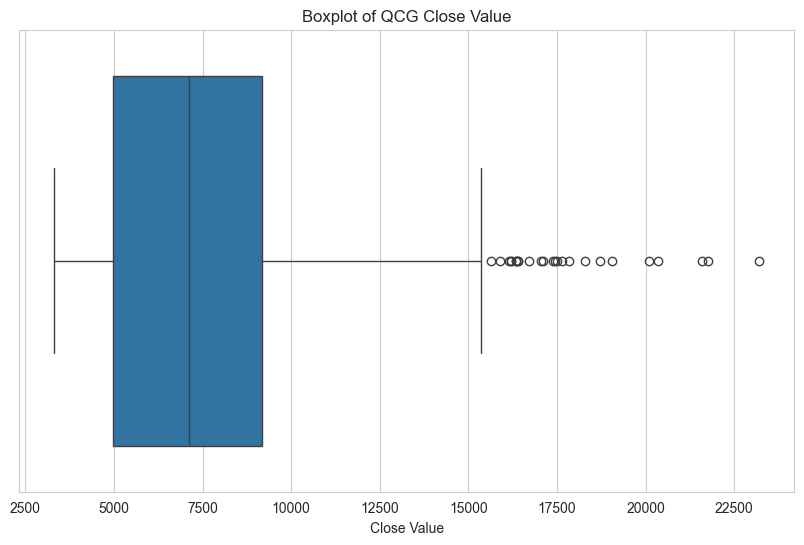
\includegraphics[width=1\textwidth]{bibliography/Figure/QCGboxplot.png}
  \caption{QCG stock price's boxplot}
  \label{fig:1}
  \end{minipage}
  \hfill
  \begin{minipage}{0.23\textwidth}
  \centering
  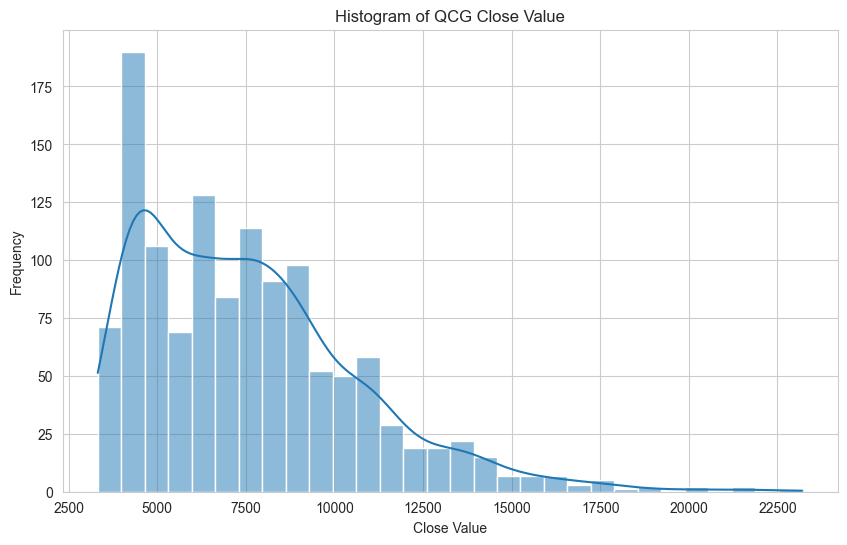
\includegraphics[width=1\textwidth]{bibliography/Figure/QCGhist.png}
  \caption{QCG stock price's histogram}
  \label{fig:2}
  \end{minipage}
\end{figure}

\begin{figure}[H]
  \centering
  \begin{minipage}{0.23\textwidth}
  \centering
  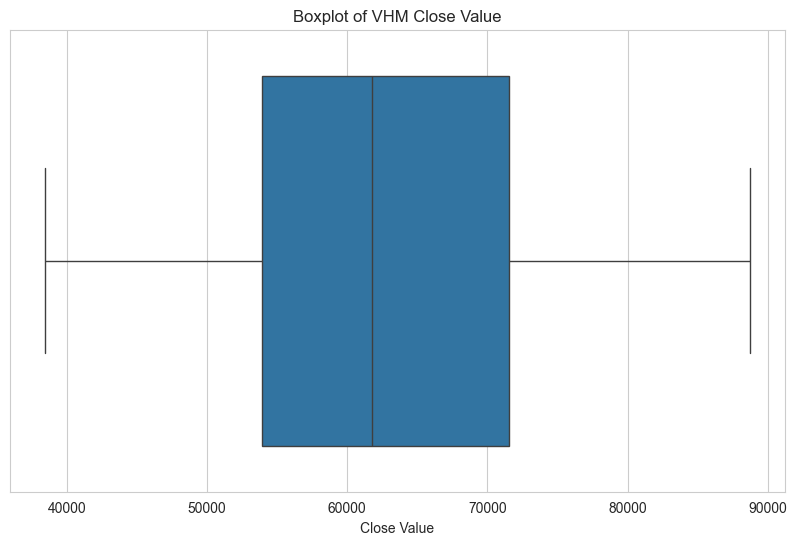
\includegraphics[width=1\textwidth]{bibliography/Figure/VHMBoxPlot.png}
  \caption{VHM stock price's boxplot}
  \label{fig:1}
  \end{minipage}
  \hfill
  \begin{minipage}{0.23\textwidth}
  \centering
  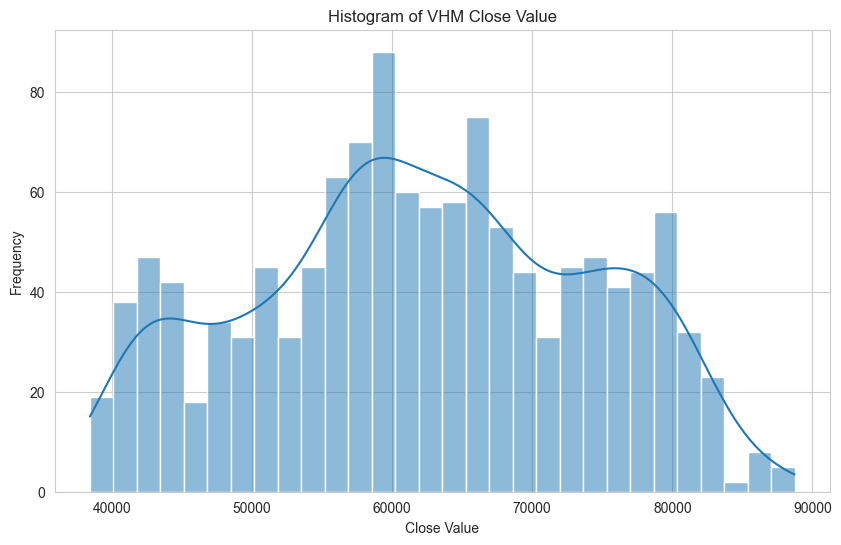
\includegraphics[width=1\textwidth]{bibliography/Figure/VHMHistogram.png}
  \caption{VHM stock price's histogram}
  \label{fig:2}
  \end{minipage}
\end{figure}

\begin{figure}[H]
  \centering
  \begin{minipage}{0.23\textwidth}
  \centering
  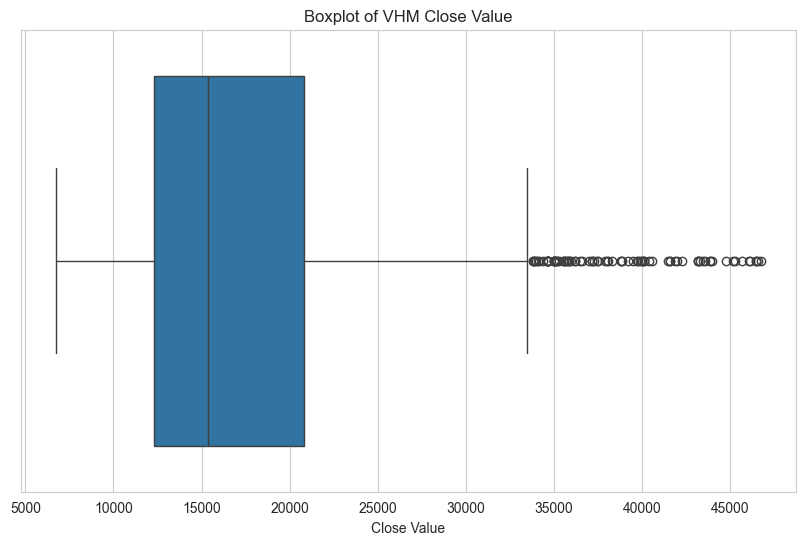
\includegraphics[width=1\textwidth]{bibliography/Figure/DXGBoxPlot.png}
  \caption{DXG stock price's boxplot}
  \label{fig:1}
  \end{minipage}
  \hfill
  \begin{minipage}{0.23\textwidth}
  \centering
  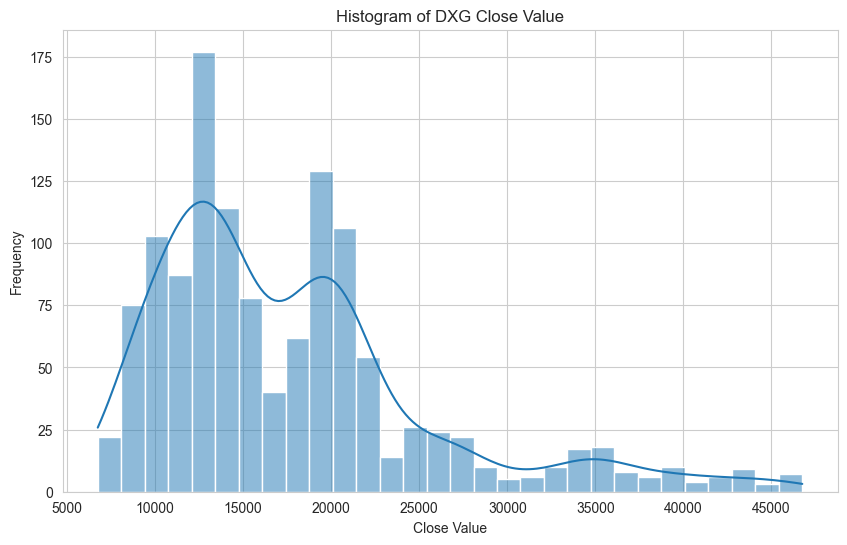
\includegraphics[width=1\textwidth]{bibliography/Figure/DXGHistogram.png}
  \caption{DXG stock price's histogram}
  \label{fig:2}
  \end{minipage}
\end{figure}


\section{Methodology}
\subsection{Data Preprocessing}
The initial dataset of daily closing stock prices was incomplete, lacking data for weekends and potentially other non-trading days, resulting in a non-consecutive time series. Recognizing the importance of a continuous time series for accurate analysis, we took steps to fill these gaps. We assumed that the market doesn't experience significant changes over non-trading days and used the closing price of the preceding Friday to fill the missing values for weekends and holidays.

Furthermore, to enhance the predictive power of our models, we calculated several technical indicators from the closing prices. These indicators included Simple Moving Average (SMA), Exponential Moving Average (EMA), Relative Strength Index (RSI), Moving Average Convergence Divergence (MACD), Bollinger Bands (BB), Average True Range (ATR), and On-Balance Volume (OBV). These widely-used indicators provide valuable information about market trends, momentum, and volatility, serving as potential predictors in our linear regression model.

By addressing the missing data and incorporating technical indicators, we created a more comprehensive and informative dataset for our subsequent analysis. This enhanced dataset enabled us to explore the relationships between stock prices and various market factors, ultimately contributing to the development of more accurate predictive models.
\subsection{Linear Regression}
A linear regression model was employed to analyze the relationship between the closing price of real estate company stocks and various technical indicators. Linear regression is a statistical method that models the linear relationship between a dependent variable and one or more independent variables. In this context, the closing price of real estate stocks was chosen as the dependent variable, while several technical indicators derived from the stock's price and volume data were considered as potential independent variables.

The mathematical representation of a multiple linear regression model is as follows:
\[Y=\beta_0+\beta_1X_1+\beta_2X_2+\cdots+\beta_kX_k+\varepsilon\]
Where:\\
	\indent\textbullet\ Y is the predicted closing price of the real estate stock. \\
	\indent\textbullet\ \(X_1, X_2, \ldots, X_k\) are the independent (explanatory) variables.\\
	\indent\textbullet\ \(\beta_0\) is the intercept term.\\
	\indent\textbullet\ \(\beta_1,..., \beta_k\) are the regression coefficients for the independent variables.\\
	\indent\textbullet\ \(\varepsilon\) is the error term.
  
  The dataset used for this analysis included stock price data for various real estate companies, spanning a specific time period. The dataset included various technical indicators such as Simple Moving Average (SMA), Exponential Moving Average (EMA), Relative Strength Index (RSI), Moving Average Convergence Divergence (MACD), Bollinger Bands (BB\_High, BB\_Middle, BB\_Low), Average True Range (ATR), and On-Balance Volume (OBV). These indicators were selected as potential independent variables due to their established relevance in technical stock analysis.

Given the high correlations between the \textit{Close} price and other price-based indicators (\textit{Open}, \textit{High}, \textit{Low}, \textit{SMA\_20}, \textit{EMA\_20}, \textit{BB\_High}, \textit{BB\_Middle}, \textit{BB\_Low}), we will exclude these to avoid multicollinearity issues. The remaining indicators (\textit{Volume}, \textit{Change \%}, \textit{RSI}, \textit{MACD}, \textit{MACD\_Signal}, \textit{MACD\_Diff}, \textit{ATR}, \textit{OBV}) will be considered as potential independent variables in the linear regression model. 

\begin{table}[ht]
\centering
\caption{Correlation Matrix of Filtered Data}
\label{tab:correlation_matrix}
\input{}
\end{table}

The model was then trained using the preprocessed dataset, and its performance was evaluated using appropriate metrics such as Mean Squared Error (MSE), R-squared, and adjusted R-squared.

The choice of independent variables for the final model was guided by the correlation matrix (Table~\ref{tab:correlation_matrix}), which revealed the strength and direction of linear relationships between the closing price and each indicator. Variables exhibiting higher correlation with the closing price were considered more influential and were prioritized for inclusion in the model.

By analyzing the estimated coefficients (\( \beta_1, \beta_2, ..., \beta_n \)) of the linear regression model, we can quantify the impact of each technical indicator on the predicted closing price of real estate stocks. This analysis provides valuable insights into the factors that drive the stock's price movements and can inform investment decisions.
  \subsection{ARIMA}
  \subsection{RNN}
  \subsection{GRU}
  % LSTM Introduction
  \subsection{Long Short Term Memory (LSTM)}

   Long Short Term Memory networks (LSTM), often known as LSTMs, are a special type of recurrent neural network (RNN) with the ability to learn and remember long-term dependencies. LSTMs were introduced by Hochreiter and Schmidhuber in 1997, and have since been refined and developed further by many researchers and experts in the field. Thanks to their exceptional performance on various tasks, LSTMs have become increasingly popular.

  LSTMs are designed to address the problem of long-term dependencies. Retaining information over extended periods is an inherent characteristic of LSTMs, requiring no special training to achieve this capability. In other words, the ability to remember long-term information is built into LSTMs.

  Unlike traditional RNNs, which have a simple structure with a single tanh activation layer, LSTMs have a more complex chain-like structure, with modules that contain up to four layers interacting in a special way.

  \noindent 
  \textbf{In the \(t\)-th state of the LSTM model:}

\textbf{Output}: \(c_t\), \(h_t\), where \(c\) is the cell state, and \(h\) is the hidden state.

\textbf{Input}: \(c_{t-1}\), \(h_{t-1}\), \(x_t\), where \(x_t\) is the input at state \(t\) of the model, and \(c_{t-1}\) and \(h_{t-1}\) are the outputs from the previous layer. The hidden state \(h\) is similar to \(s\) in RNN, while \(c\) is the unique aspect of LSTM.

\textbf{Reading the diagram}: The symbols \(\sigma\) and tanh indicate that the step uses the sigmoid and tanh activation functions, respectively. The multiplication is element-wise, and the addition is matrix addition.

\textbf{Gates}: \(f_t\), \(i_t\), \(o_t\) correspond to the forget gate, input gate, and output gate, respectively.

\begin{figure}[H]
  \centering
  \begin{minipage}{0.5\textwidth}
    \centering
    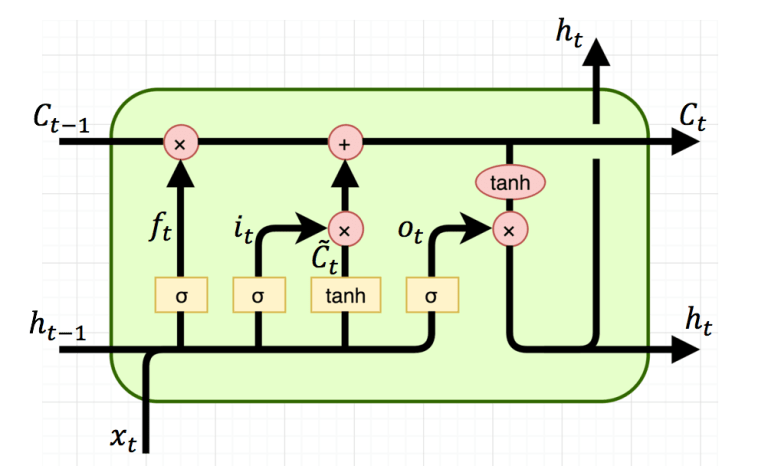
\includegraphics[width=\textwidth]{bibliography/Figure/LSTM Model.png}
    \caption{LSTM Model}
    \label{fig:1}
  \end{minipage}
\end{figure}



\noindent \textbullet \textbf{ Forget gate}:
\[
f_t = \sigma(U_f \cdot x_t + W_f \cdot h_{t-1} + b_f)
\]

\noindent \textbullet \textbf{ Input gate}:
\[
i_t = \sigma(U_i \cdot x_t + W_i \cdot h_{t-1} + b_i)
\]

\noindent \textbullet \textbf{ Output gate}:
\[
o_t = \sigma(U_o \cdot x_t + W_o \cdot h_{t-1} + b_o)
\]

Thus, the expressions for each gate of the LSTM illustrate how each gate manages the information flowing in and out of the model's states.


  % TimesNet Introduction
  \subsection{TimesNet}
  \subsection{Fast Fourier Transform Forecasting Model (FFT)}
  \subsection{Random Forest}

 
\section{Result}
Placeholder line
\subsection{Evaluation Methods}
\textbf{Mean Percentage Absolute Error} (MAPE): is the average percentage error in a set of predicted values.\\
\[MAPE=\frac{100\%}{n}  \sum_{i=1}^{n} |y_i-\hat{y_i} |  = 1 \]\\
\textbf{Root Mean Squared Error} (RMSE): is the square root of average value of squared error in a set of predicted values.\\
\[RMSE=\sqrt{\sum_{i=1}^{n} \frac{(\hat{y_i}-y_i )^2}{n} }\]\\
\textbf{Mean Absolute Error} (MSLE):is the relative difference between the log-transformed actual and predicted values.\\
\[MSLE=\frac{1}{n}\sum_{i=1}^{n}(log(1+\hat{y_i})-log(log(1+y_i))^2\]
Where: \\
	\indent\textbullet\ \(n\) is the number of observations in the dataset.\\
	\indent\textbullet\ \(y_i\)  is the true value.\\
	\indent\textbullet\ \(\hat{y_i}\) is the predicted value.
\subsection{DXG Dataset} 
\begin{table}[H]
  \begin{tabular}{|c|c|c|c|c|}
  \hline
  \multicolumn{1}{|l|}{Dataset} & \multicolumn{1}{l|}{Train-Test-Validate} & \multicolumn{1}{l|}{RMSE} & \multicolumn{1}{l|}{MDA} & \multicolumn{1}{l|}{MAPE} \\ \hline
  \multirow{3}{*}{DXG}          & 7-2-1                                    & 251.28                    & 44.95                    & 3.82                      \\ \cline{2-5} 
                                & 7.5-1.5-1                                & 250.04                    & 48.39                    & 3.59                      \\ \cline{2-5} 
                                & 8-1.50.5                                 & 167.48                    & 49.68                    & 2.02                      \\ \hline
  \end{tabular}
  \caption{DXG Dataset's Evaluation}
    \label{vcbresult}
  \end{table}


\subsection{VHM dataset} 



\subsection{QCG dataset} 

\section{Conclusion}
 Placeholder line
\subsection{Summary}
Placeholder
\subsection{Future Considerations}
Placeholder line
\section*{Acknowledgment}
\addcontentsline{toc}{section}{Acknowledgment}
Placeholder line

%% UNCOMMENT these lines below (and remove the 2 commands above) if you want to embed the bibliografy.
\begin{thebibliography}{00}
\bibitem{b1} Hind Daori, Alanoud Alanazi, Manar Alharthi, Ghaida Alzahrani
 ,  ''Predicting Stock Prices Using the Random ForestClassifier'', November, 14th, 2022.
\bibitem{b2} Hugo Souto, 2023, ''TimesNet for Realized Volatility Prediction
''.
\bibitem{b3} Bohumil Stádník, Jurgita Raudeliuniene, Vida Davidavičienė , 2016. Fourier Analysis For Stock Price Forecasting: Assumption And Evidence .

\end{thebibliography}
%%%%%%%%%%%%%%%


\EOD

\end{document}
